\en

\section{Tool architecture}
\label{subsec:architecture}

The Preprocessor contains two main components, the Function Breaker and the Code Duplication Finder. 
The flow of how the Preprocessor works is as follow: Function Parser receives the codebase the user is interested in,
extracts the functions of the codebase along with metadata, and creates a new temporary codebase where the functions extracted become new code files. 
The Code Duplication Finder iterates over every pair of files in the Temporary Codebase, checks if they are code clones, and, 
if so, saves them in the Code Duplication Database, which is a text file that stores every code duplication as a triple 
\textbf{<function1,function2,similarity>}, where \textbf{function1} and \textbf{function2} are the functions that are duplicates 
of each other, and \textbf{similarity} is the metric given by the code duplication detection method utilized in the Code Duplication Finder. ,

The Query Responder consumes the Temporary Codebase and the Code Duplication Database to extract duplicated 
functions-related information per user request. If the user executes the Query Responder without executing the 
Preprocessor, the Query Responder calls the Preprocessor to create the required artifacts.

Figure \ref{fig:diagram} illustrates the tool architecture. An explanation of how each component works is provided in this section.

\begin{figure}
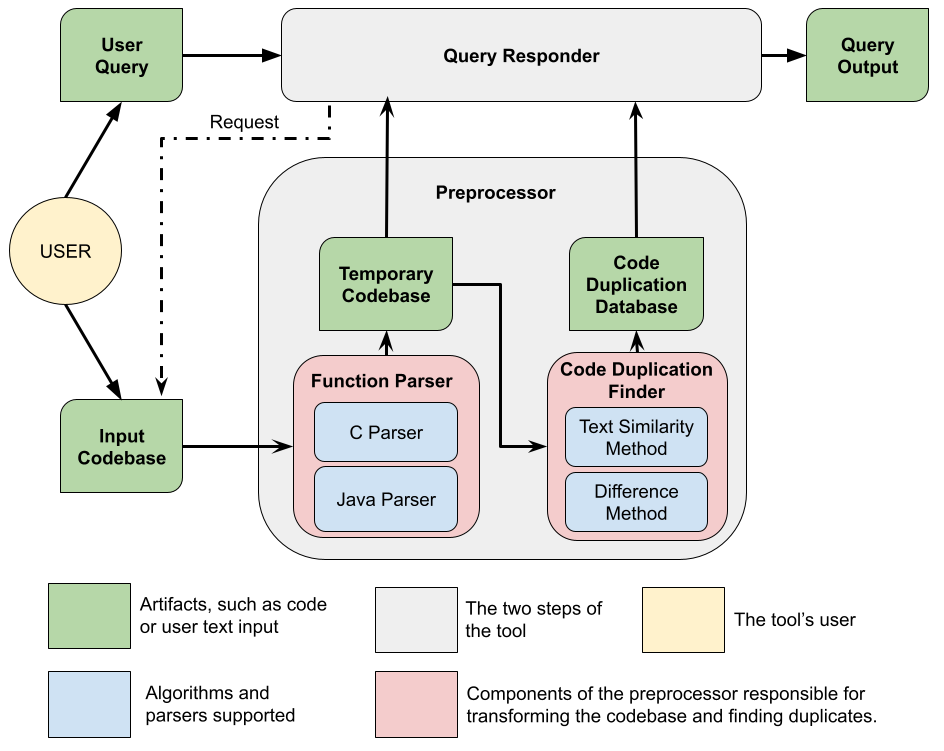
\includegraphics[scale=0.4]{diagrama_mestrado}
\caption{Architecture diagram demonstrating the relationship between the tool components.}
\label{fig:diagram}
\end{figure}

\subsection{Input codebase}

The input codebase is a folder on the machine running the tool. All files in the codebase that are not source code files from a programming language supported by the tool are ignored. The tool validates support for a source file by analyzing its file extension.

\subsection{Function Parser}

The Function Parser receives the input codebase and transforms it into the temporary codebase. The Function Parser iterates through every source code file from the programming language it supports and uses a specific programming language function extractor to extract every function in the file. For each function extracted, two new source code files and a metadata file are created in the temporary codebase, represented by the pair \textbf{<file name, function name>}, the source code file of the function, and the proper function. The first new source code file contains the function's body from the function it represents, while the other new source code file contains the function's signature. The metadata file contains additional relevant information about the function, such as the function name, the line where the function signature starts in the source code file, and the line where the function's body ends in the source code file. The programming languages supported at the moment are C and Java. Figure \ref{fig:transform} illustrates an example of a function transformation into the temporary codebase.

\begin{figure}
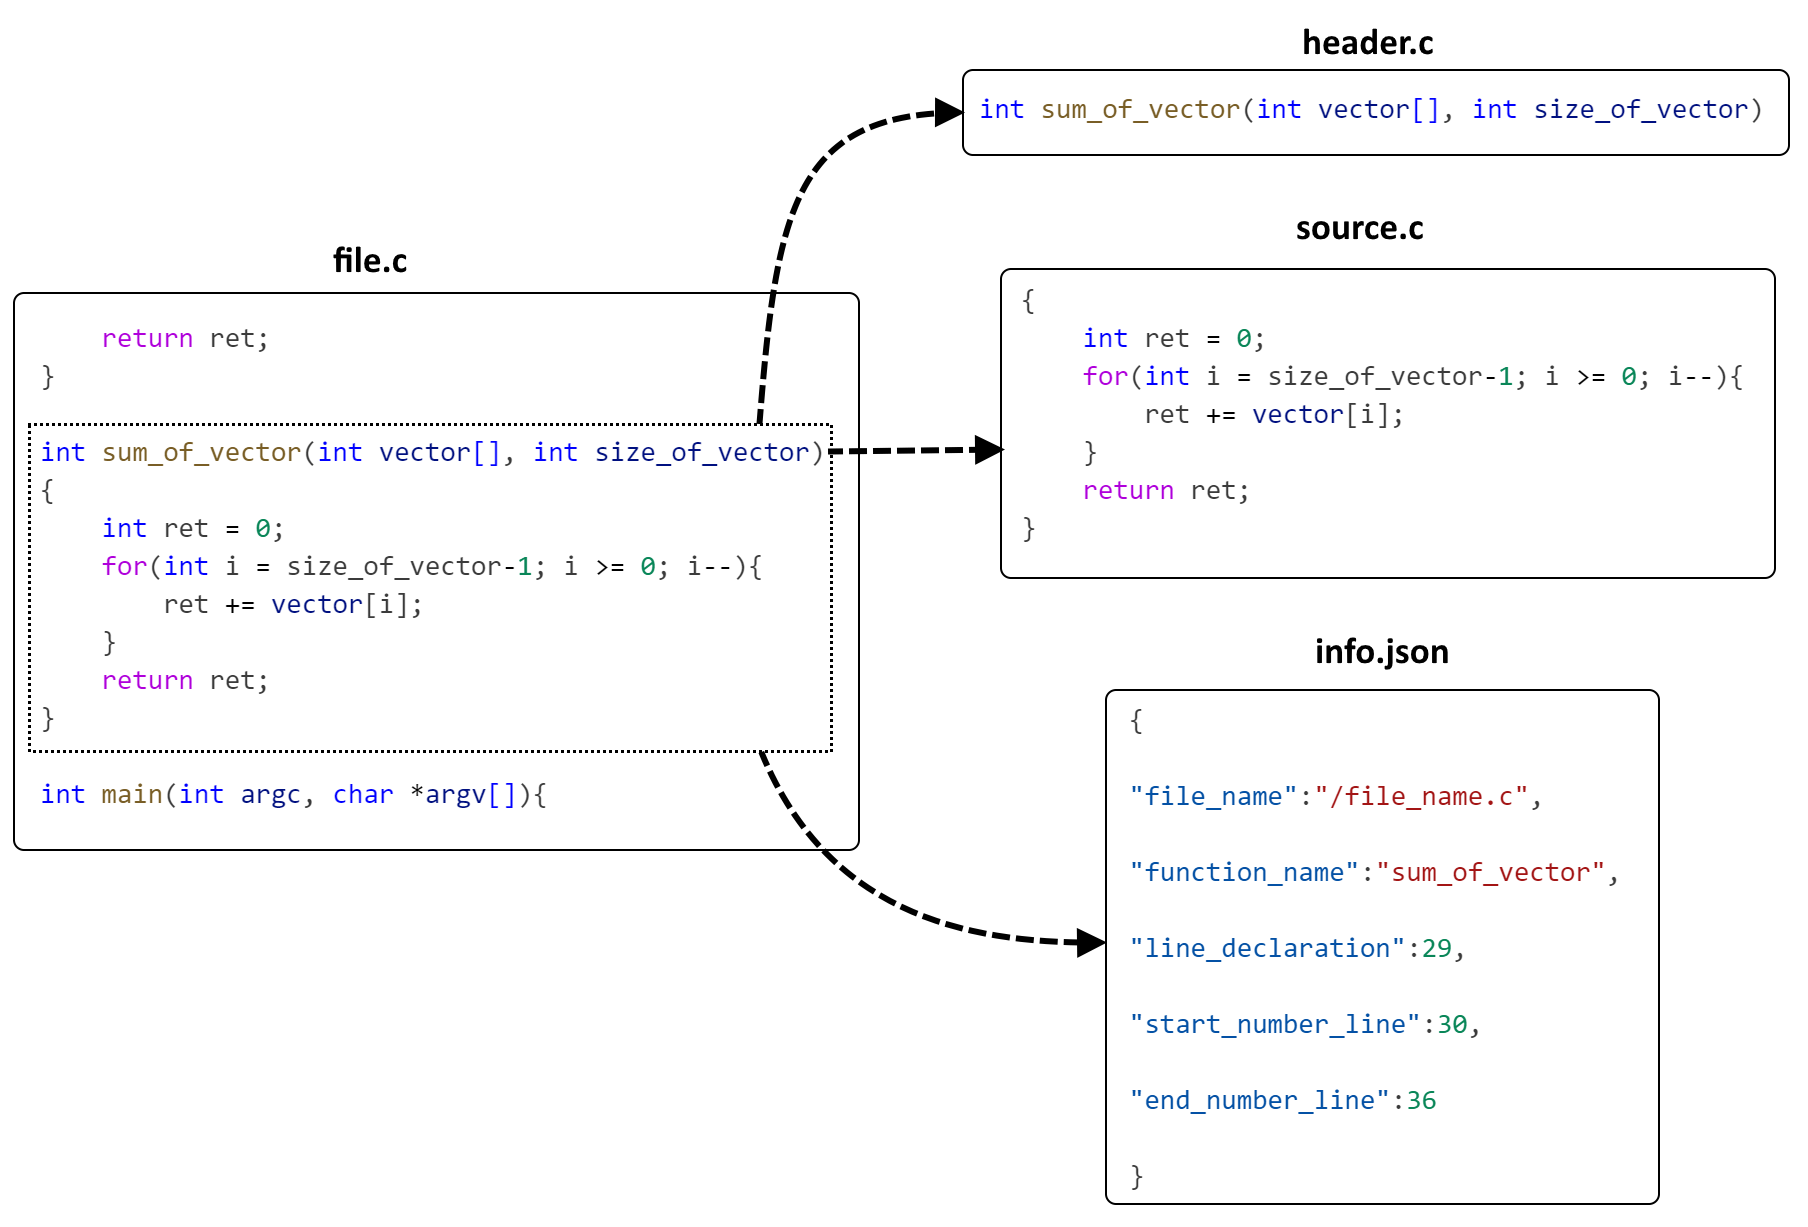
\includegraphics[scale=0.3]{example_function_parser/example_parser}
\caption{Transformation of a function into the temporary codebase}
\label{fig:transform}
\end{figure}

Regarding the programming language's function extractor, we approached this problem so that anyone comfortable with a language can adapt our approach to their specific programming language. Usually, code blocks can be easily extracted from source code files, independently if the code blocks are defined by curly brackets or by indentation, and it is possible to infer if they represent a function's body given their depth in the code context and a few lines before the start of the code block. We followed this approach to implement the function extractor for the supported languages. As an alternative approach, we can build the syntax tree \citep{compiler} of the programming language and use it to extract the functions, which is a more complex task than our approach. For the programming languages that we support, we implemented them as follows:

\subsubsection{C Programming Language}

For a source file in the C programming language, we extract the code blocks with depth 0; 
as per the programming language’s grammar, functions are defined in a global context at depth 0. 
To extract the code blocks, we first need to identify the portions of code that are comments or 
\textit{\#define} directives and mark them as irrelevant. After that, it is simple work to find 
the curly brackets in depth 0, and with that, we find the body of the functions.

To extract the header of the functions, we start at the open curly brackets and go back in the 
source file considering the programming language grammar and the portions of code that have been 
marked as irrelevant because of comments and \textit{\#define} directives.
There are other elements in depth zero that are not functions. We analyze whether the code blocks 
are functions at the same time that we extract the header of the code block.

\subsubsection{Java Programming Language}

For the Java programming language, we have decided to implement a more straightforward approach 
that does not support the programming language completely, as the only Java codebase explored in 
this work is the BigCloneBench \citep{bigclonebench}, and the approach implemented covers the 
needs of this codebase.

For a source file in Java, we extract the code blocks with depth one and some code lines before 
defining them. Then, we check if the code blocks are functions by analyzing whether the first 
non-empty character before the curly brackets of the code block is a closing parenthesis.

As per Java’s grammar, functions are defined inside classes and can exist at different depths. 
As Java accepts inner classes, this approach does not work with inner classes. The challenge 
to implementing a more generic approach is that other elements of depth two or deeper, such 
as for-loops, can follow the closing parenthesis pattern, necessitating a better analysis of 
these elements. The BigCloneBench \citep{bigclonebench} does not contain inner classes.

\subsection{Temporary codebase}

The temporary codebase is a transformation of the input codebase performed by the Function Parser. Each function in the input codebase is represented in the temporary codebase as three files. Descriptions of these files are provided below, with examples shown in Figure \ref{fig:transform}.

\begin{itemize}
	\item \textbf{Header file}: This file contains the signature of the function it represents.
	\item \textbf{Source file}: This file contains the body of the function it represents.
	\item \textbf{Info file}: This file contains metadata about the function, including the function name, the file that contains the function, the file's relative path to the input codebase, the line where the function's signature starts, the line where the function body begins, the line where the function's body ends, and whether there is a line break between the end of the function's signature and the start of the function's body.
\end{itemize}

\subsection{Code Duplication Finder}

\label{subsec:code_finder}

The Code Duplication Finder iterates through every pair of source code files in the temporary codebase, representing 
functions from the input codebase. For each pair of files, we execute a code duplication detection method that computes 
a metric measuring how similar the pair of files is, which we refer to as similarity. 
If the similarity is greater than or equal to the minimum similarity threshold 
(a parameter provided by the user during the Preprocessor), we store this pair of functions along with its 
similarity in the Code Duplication Database.

We implemented two methods for code duplication detection in the tool, which the user can 
choose to use. The first method is based on text similarity, and the second is simpler and 
based on the number of equal lines. The experiments and tests in this research were done 
using the text similarity method. The purpose of the second method is to demonstrate that 
the tool can have multiple duplication detection methods.

\subsubsection{Text Similarity Method}

For the text similarity method, we treat the source code files 
as text and apply the TF-IDF vector embedding method implemented by the 
Gensim library \citep{gensim}, then compute cosine similarity as the 
similarity metric.

This method was chosen for its claimed performance, 
programming language independence, and the fact that it does not require 
compilable code, which is expected in the temporary codebase, as it does 
not contain complete code artifacts. We expect our method to yield good 
results for Type-1 and Type-2 code duplication types while performing 
poorly for the other types. It is possible to change the code duplication 
detection method to one of the state-of-the-art methods if needed.

\cite{platistool} implemented this code duplication detection method and 
released it under the MIT license \citep{mitlicense}. We adapted his 
implementation to fit our tool's expected input and output formats. 
Switching the duplication detection method is feasible, similar to how 
we adapted Plates' implementation.

\subsubsection{Difference Method}

For the difference method, 
we implemented a method that considered the number of exactly equal lines between two functions.
For two functions \textit{function1} and \textit{function2}, let $NL_1$ be the number of lines in \textit{function1},
$NL_2$ be the number of lines in \textit{function2}, and $EQ$ be the number of equal lines between \textit{function1} and
\textit{function2}, we compute the similarity with the formula:

$$\frac{2 \cdot EQ}{NL_1 + NL_2}$$

This code duplication method is considerably simpler and more explainable than the text similarity method, 
as the metric is the ratio of common lines between the two functions. To compute the number of equal lines, we use
the \textit{diff} command built-in in the Linux environment \citep{diffcommand}.

We did not test the Diff method during the tool evaluation and other phases of this research. 
We implemented the technique to show that a tool can have multiple duplication detection methods.

\subsection{Code Duplication Database}

The Code Duplication Database is a text file that contains the duplicated pairs of functions found by the Code Duplication Finder. The first line of the file specifies the number of duplicated pairs. Following this, each line lists a duplicated pair, including the paths of the functions in the temporary codebase and the similarity metric of the pair.

\subsection{Preprocessor}
\label{subsec:setup}

The Preprocessor is a procedure executed by the user once per codebase. 
The Preprocessor takes the input codebase and a minimum similarity metric value for function pairs considered duplicates. 
It then runs the Function Parser and the Code Duplication Finder to create a temporary codebase and the Code Duplication Database. 
Setting a minimum similarity metric reduces the Code Duplication Database size, optimizing memory usage and the computational 
cost of the Query Responder step. For example, if this parameter does not exist and we work with a codebase of $10000$ functions, 
each with a 50-character relative path and function name, the Code Duplication Database would reach approximately $5000^2 \times 50 ~= 5$ gigabytes. 
As most function pairs are unlikely to be duplicated in large codebases, this file size can be significantly reduced.

\subsection{Query Responder}

\todo[inline]{I NEED TO CHANGE HERE}

The Query Responder step is the component the user executes multiple times to consult information about duplicated functions in a codebase processed by the Preprocessor. The Query Responder step utilizes the temporary codebase and the Code Duplication Database as inputs to answer the user's request, such as querying the total number of duplicated functions in a specific input codebase or listing duplicated functions above a certain similarity threshold. This component was developed to be extensible, allowing other queries to be easily added. Currently, the Query Responder step supports the following queries:

\begin{itemize}
	\item Number of dupliddcated functions above a similarity threshold.
	\item Number of duplicated functions equal or above a similarity threshold.
	\item List of duplicated functions above a similarity threshold.
	\item List of duplicated functions equal to or above a similarity threshold.
\end{itemize}
